 
\section{Praktika enkonduko}
\subsection{Uzantkontoj}
%%%>>>>>>>>>>>>>>>>>>>>>>>>>>>>>>>>>>>>>>>>>>>>>>>>>>>>>>>>>>>>>>>>>>>>>>>>>>>>>>>>>>>>>>>>>>>>>>
  \begin{frame}
    \frametitle{Ensalutu en trellon}

	Uzu sian propran konton aŭ uzu unu de la subaj:

%	\begin{tabular}{ | c | c | }
%	\hline                       
%		anaso_trejnanto gmail.com & 2anasoj \\
%		alaudo_trejnanto gmail.com & 2alaudoj \\
%		najtingalo_trejnanto gmail.com & 2najgingaloj \\
%		kolombo_trejnanto gmail.com & 2kolomboj\\
%	\hline  
%	\end{tabular}

\end{frame}
%%%<<<<<<<<<<<<<<<<<<<<<<<<<<<<<<<<<<<<<<<<<<<<<<<<<<<<<<<<<<<<<<<<<<<<<<<<<<<<<<<<<<<<<<<<<<<<<<

%%%>>>>>>>>>>>>>>>>>>>>>>>>>>>>>>>>>>>>>>>>>>>>>>>>>>>>>>>>>>>>>>>>>>>>>>>>>>>>>>>>>>>>>>>>>>>>>>
  \begin{frame}
    \frametitle{Fulmklavoj}
    	\begin{columns}
    \column{0.6\textwidth}
	
	Estas malmultaj, sed ege utilaj.
    
	\begin{itemize}
		\item Per klavo ? vi povas rigardi fulmklavaron.
		\item Tre indas tion fari ofte kaj lerni paŝo post paŝo.
	\end{itemize}
    
    	
	\column{0.4\textwidth}
    
    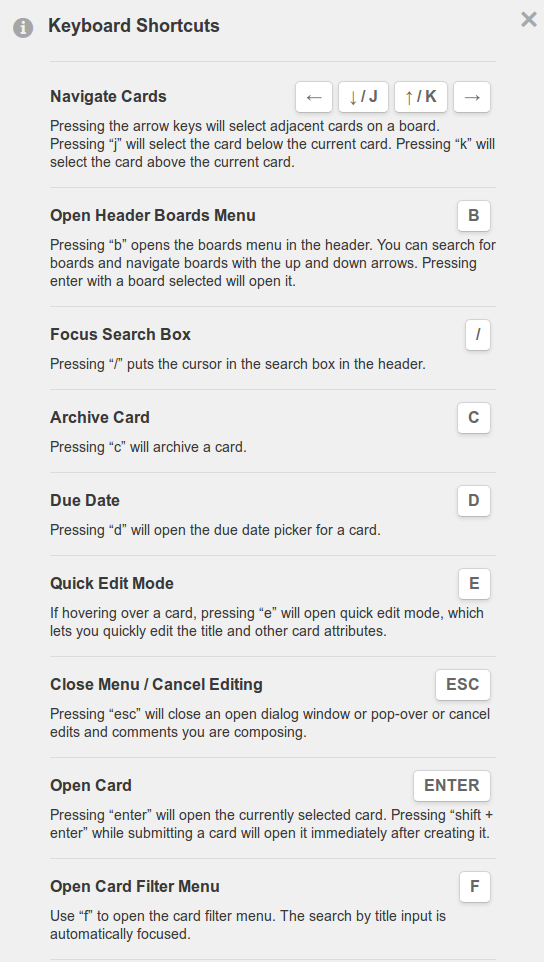
\includegraphics[scale=0.2]{ekranoj/fulmklavaro}
	
	\end{columns}
	
	
  \end{frame}
%%%<<<<<<<<<<<<<<<<<<<<<<<<<<<<<<<<<<<<<<<<<<<<<<<<<<<<<<<<<<<<<<<<<<<<<<<<<<<<<<<<<<<<<<<<<<<<<<




%%%>>>>>>>>>>>>>>>>>>>>>>>>>>>>>>>>>>>>>>>>>>>>>>>>>>>>>>>>>>>>>>>>>>>>>>>>>>>>>>>>>>>>>>>>>>>>>>
  \begin{frame}
    \frametitle{Limdatoj}

    \begin{columns}
    \column{0.6\textwidth}
    
    Tre utilas. Oni ankaŭ ricevas sciigon unu tago antaŭ ĝi.
    
    	
	\column{0.4\textwidth}
    
    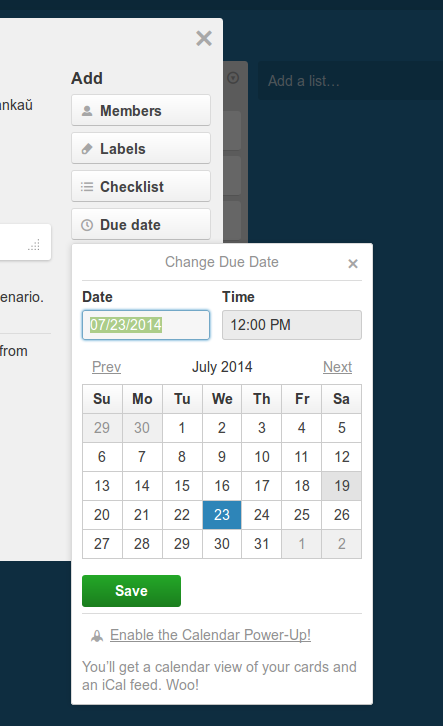
\includegraphics[scale=0.2]{ekranoj/limdato}
	
	\end{columns}
	
	
	
  \end{frame}
%%%<<<<<<<<<<<<<<<<<<<<<<<<<<<<<<<<<<<<<<<<<<<<<<<<<<<<<<<<<<<<<<<<<<<<<<<<<<<<<<<<<<<<<<<<<<<<<<



%%%>>>>>>>>>>>>>>>>>>>>>>>>>>>>>>>>>>>>>>>>>>>>>>>>>>>>>>>>>>>>>>>>>>>>>>>>>>>>>>>>>>>>>>>>>>>>>>
  \begin{frame}
    \frametitle{Nomo de kartoj}
		
	Trello havas tre potencan serĉilon. La nomo estu ŝerĉebla post du jaroj.
	
	Ezkemple, anstataŭ "Paperaĵoj" uzu "Pruviloj de la vojaĝo al Italio".
  \end{frame}
%%%<<<<<<<<<<<<<<<<<<<<<<<<<<<<<<<<<<<<<<<<<<<<<<<<<<<<<<<<<<<<<<<<<<<<<<<<<<<<<<<<<<<<<<<<<<<<<<



%%%>>>>>>>>>>>>>>>>>>>>>>>>>>>>>>>>>>>>>>>>>>>>>>>>>>>>>>>>>>>>>>>>>>>>>>>>>>>>>>>>>>>>>>>>>>>>>>
  \begin{frame}
    \frametitle{Markolistoj}
		
		\begin{center}
		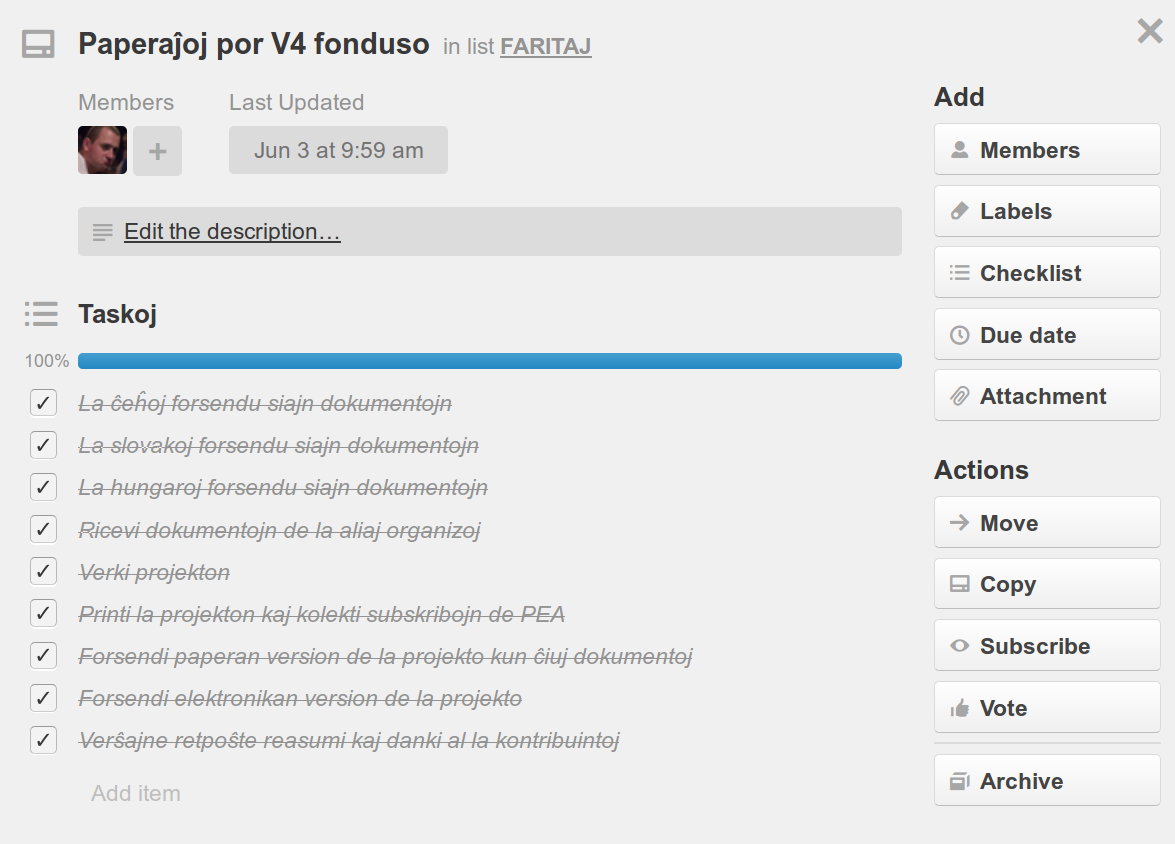
\includegraphics[scale=0.222]{ekranoj/markolistoj}
		\end{center}
	
  \end{frame}
%%%<<<<<<<<<<<<<<<<<<<<<<<<<<<<<<<<<<<<<<<<<<<<<<<<<<<<<<<<<<<<<<<<<<<<<<<<<<<<<<<<<<<<<<<<<<<<<<



%%%>>>>>>>>>>>>>>>>>>>>>>>>>>>>>>>>>>>>>>>>>>>>>>>>>>>>>>>>>>>>>>>>>>>>>>>>>>>>>>>>>>>>>>>>>>>>>>
  \begin{frame}
    \frametitle{Markolistoj + Mencioj}
    
	\begin{center}
    	Atentu: \alert{tio ne produktas sciigojn!}
	\end{center}
		
	\begin{center}
		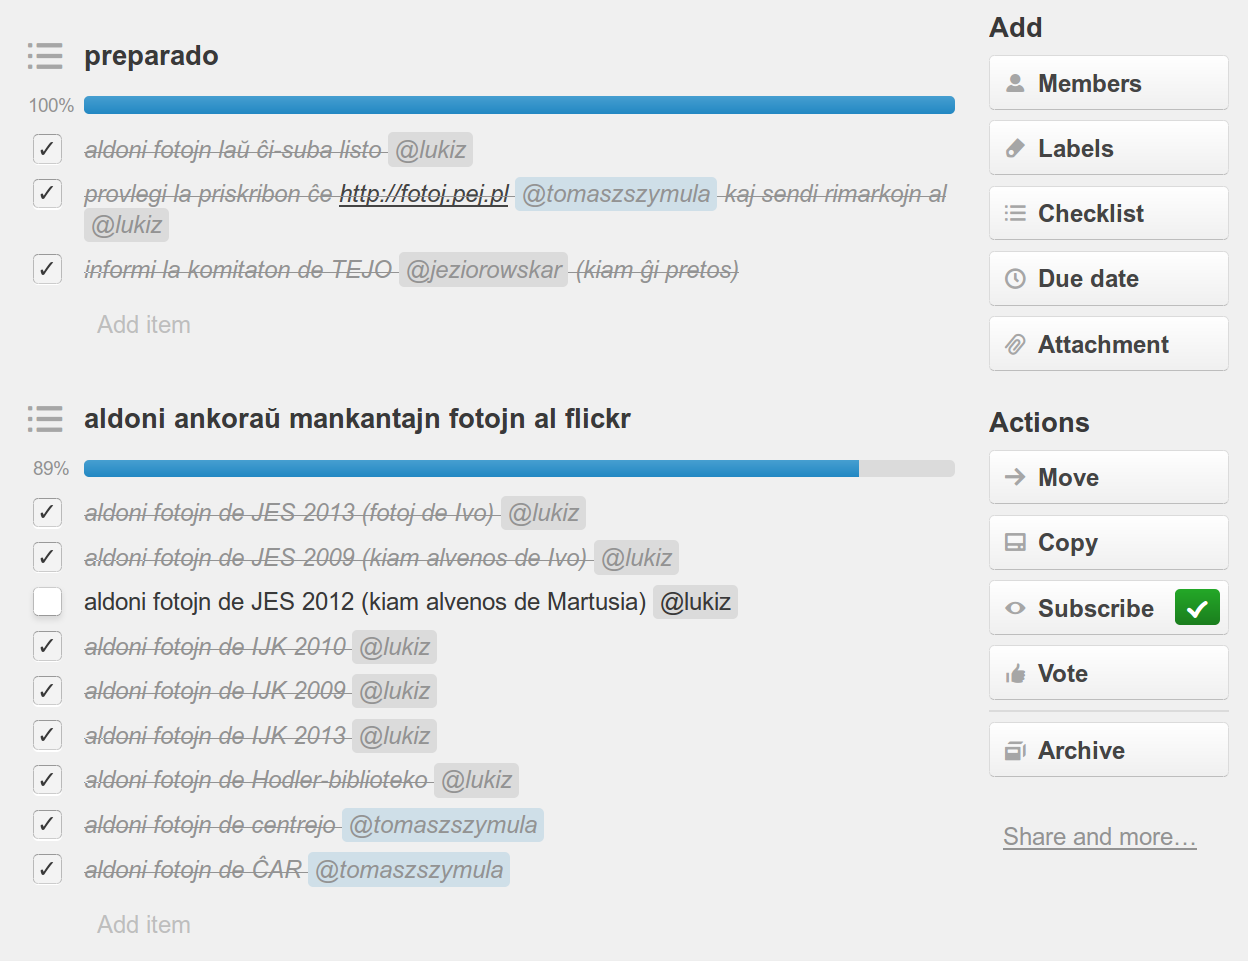
\includegraphics[scale=0.175]{ekranoj/markolistoj-kun-mencioj}
	\end{center}
	
  \end{frame}
%%%<<<<<<<<<<<<<<<<<<<<<<<<<<<<<<<<<<<<<<<<<<<<<<<<<<<<<<<<<<<<<<<<<<<<<<<<<<<<<<<<<<<<<<<<<<<<<<


\subsection{Para klakado}
%%%>>>>>>>>>>>>>>>>>>>>>>>>>>>>>>>>>>>>>>>>>>>>>>>>>>>>>>>>>>>>>>>>>>>>>>>>>>>>>>>>>>>>>>>>>>>>>>
  \begin{frame}
    \frametitle{Pariĝu!}
    Decidu kiu unue estos kunordiganto (poste la roloj interŝanĝiĝos, ne tiom gravas).
    
    Ambaŭ personoj havu iun ajn aliron al Trello: telefono, tableto aŭ komputilo.
    
    Se iloj mankos reuzu, ni atendos.
    
    Mi petegas: ne malpurigu la komputilon! :-)
    
  \end{frame}
%%%<<<<<<<<<<<<<<<<<<<<<<<<<<<<<<<<<<<<<<<<<<<<<<<<<<<<<<<<<<<<<<<<<<<<<<<<<<<<<<<<<<<<<<<<<<<<<<

%%%>>>>>>>>>>>>>>>>>>>>>>>>>>>>>>>>>>>>>>>>>>>>>>>>>>>>>>>>>>>>>>>>>>>>>>>>>>>>>>>>>>>>>>>>>>>>>>
  \begin{frame}
    \frametitle{Ekzerco}
	
	Scenariusz: jedna osoba jest diżoranto w gufujo i proponuje drugiej zjedzenia wafla z dżemem/nutellą -- zadaniem będzie przeprowadzenie śniadania przez trello (milcząc?). Potem na odwrót. Jeśli będzie za mało komputerów to na rzutniku czy coś.
    
    
%    Kunordiganto:
%        Kreu karton "manĝajho"
%        komponu la liston de la bazaj bezonataj artikoloj: pano, smirajho
%    Manĝorespondeculo
%        aldonu buteron al la listo
%        demandu la kunordiganton kiom da konfituraĵo meti sur la panon (demetu sin de la karto kaj metu la kunordiganton)
%    Kunordiganto:
%        respondu (demetu sin kaj remetu manĝrespondeculon)
%    Manĝrespondeculo:
%        eklaboru! se vi havas pliajn demandojn ("kie estas pano?") ktp
  \end{frame}
%%%<<<<<<<<<<<<<<<<<<<<<<<<<<<<<<<<<<<<<<<<<<<<<<<<<<<<<<<<<<<<<<<<<<<<<<<<<<<<<<<<<<<<<<<<<<<<<<


%%%>>>>>>>>>>>>>>>>>>>>>>>>>>>>>>>>>>>>>>>>>>>>>>>>>>>>>>>>>>>>>>>>>>>>>>>>>>>>>>>>>>>>>>>>>>>>>>
  \begin{frame}
    \frametitle{Esenco}
    
	Vi ĉiam strebu \alert{forigi sian vizaĝon de la karto} per:
    
    \begin{itemize}
    	\item plenumo de la peto/tasko,
    	\item klarigo kial ne vi taŭgas (ĉiam trovu anstataŭanton),
    	\item aliaj laŭ via kreemeco, kondiĉe ke kun \alert{fortaj argumentoj} por tio.
    \end{itemize}
    
  \end{frame}
%%%<<<<<<<<<<<<<<<<<<<<<<<<<<<<<<<<<<<<<<<<<<<<<<<<<<<<<<<<<<<<<<<<<<<<<<<<<<<<<<<<<<<<<<<<<<<<<<

